%!TEX root = ../template.tex
%%%%%%%%%%%%%%%%%%%%%%%%%%%%%%%%%%%%%%%%%%%%%%%%%%%%%%%%%%%%%%%%%%%%
%% chapter6.tex
%% NOVA thesis document file
%%%%%%%%%%%%%%%%%%%%%%%%%%%%%%%%%%%%%%%%%%%%%%%%%%%%%%%%%%%%%%%%%%%%

\typeout{NT FILE chapter6.tex}%

\chapter{Plano de Trabalho}
\label{cha:work_plan}

\glsresetall
\prependtographicspath{{Chapters/Figures/Covers/}}

\section{Plano de Execução e Consolidação do Protocolo}
\label{sec:execution_plan}

O plano de execução foca na implementação prática do protocolo proposto, na
coleta sistemática de evidências empíricas e na elaboração final da dissertação.
As etapas descritas a seguir asseguram que o protocolo seja avaliado
rigorosamente e alinhado aos princípios metodológicos estabelecidos nesta
pesquisa.

A fase inicial contempla o desenvolvimento do protocolo, permitindo a análise de
sua eficácia em organizações com diferentes graus de horizontalidade. Esta etapa
será orientada pelos seguintes objetivos:

\textbf{Desenvolvimento do Protocolo}: A configuração de ambientes de teste
incluirá simulações detalhadas que repliquem cenários organizacionais
horizontais. Essa fase buscará implementar os mecanismos essenciais do
protocolo, como sistemas de registro imutável, participação democrática e
validação descentralizada. Será assegurado que o protocolo seja adaptável às
dinâmicas de diferentes organizações, permitindo respostas adequadas a cenários
de ameaça e falhas operacionais.

\textbf{Validação Iterativa}: Os testes serão conduzidos para avaliar o
desempenho do protocolo em situações como falhas planejadas, centralização
temporária e manipulação de quórum. Esse processo permitirá a identificação de
vulnerabilidades e o refinamento contínuo de contramedidas, garantindo a
robustez e a escalabilidade do protocolo.

\textbf{Coleta de Dados Empíricos}: Durante os experimentos, serão registrados
dados quantitativos, como tempos de resposta, níveis de participação e taxas de
detecção de ameaças, além de feedback qualitativo sobre a usabilidade e clareza
do protocolo. Esses dados embasarão uma análise comparativa entre o protocolo
proposto e modelos alternativos, como o \gls{stride}, destacando diferenças na
eficácia e aplicação.

Após a coleta e análise dos dados, será conduzida a etapa de consolidação
acadêmica e redação final da dissertação. Os resultados quantitativos e
qualitativos serão integrados em uma análise abrangente, destacando a
contribuição do protocolo para a segurança e governança em organizações
horizontais. Limitações serão discutidas de forma crítica, com recomendações
para aplicações futuras e possíveis adaptações do protocolo a outros cenários.

\section{Gantt Chart}
\label{sec:gantt_chart}


\begin{figure}[htbp]
  \centering
  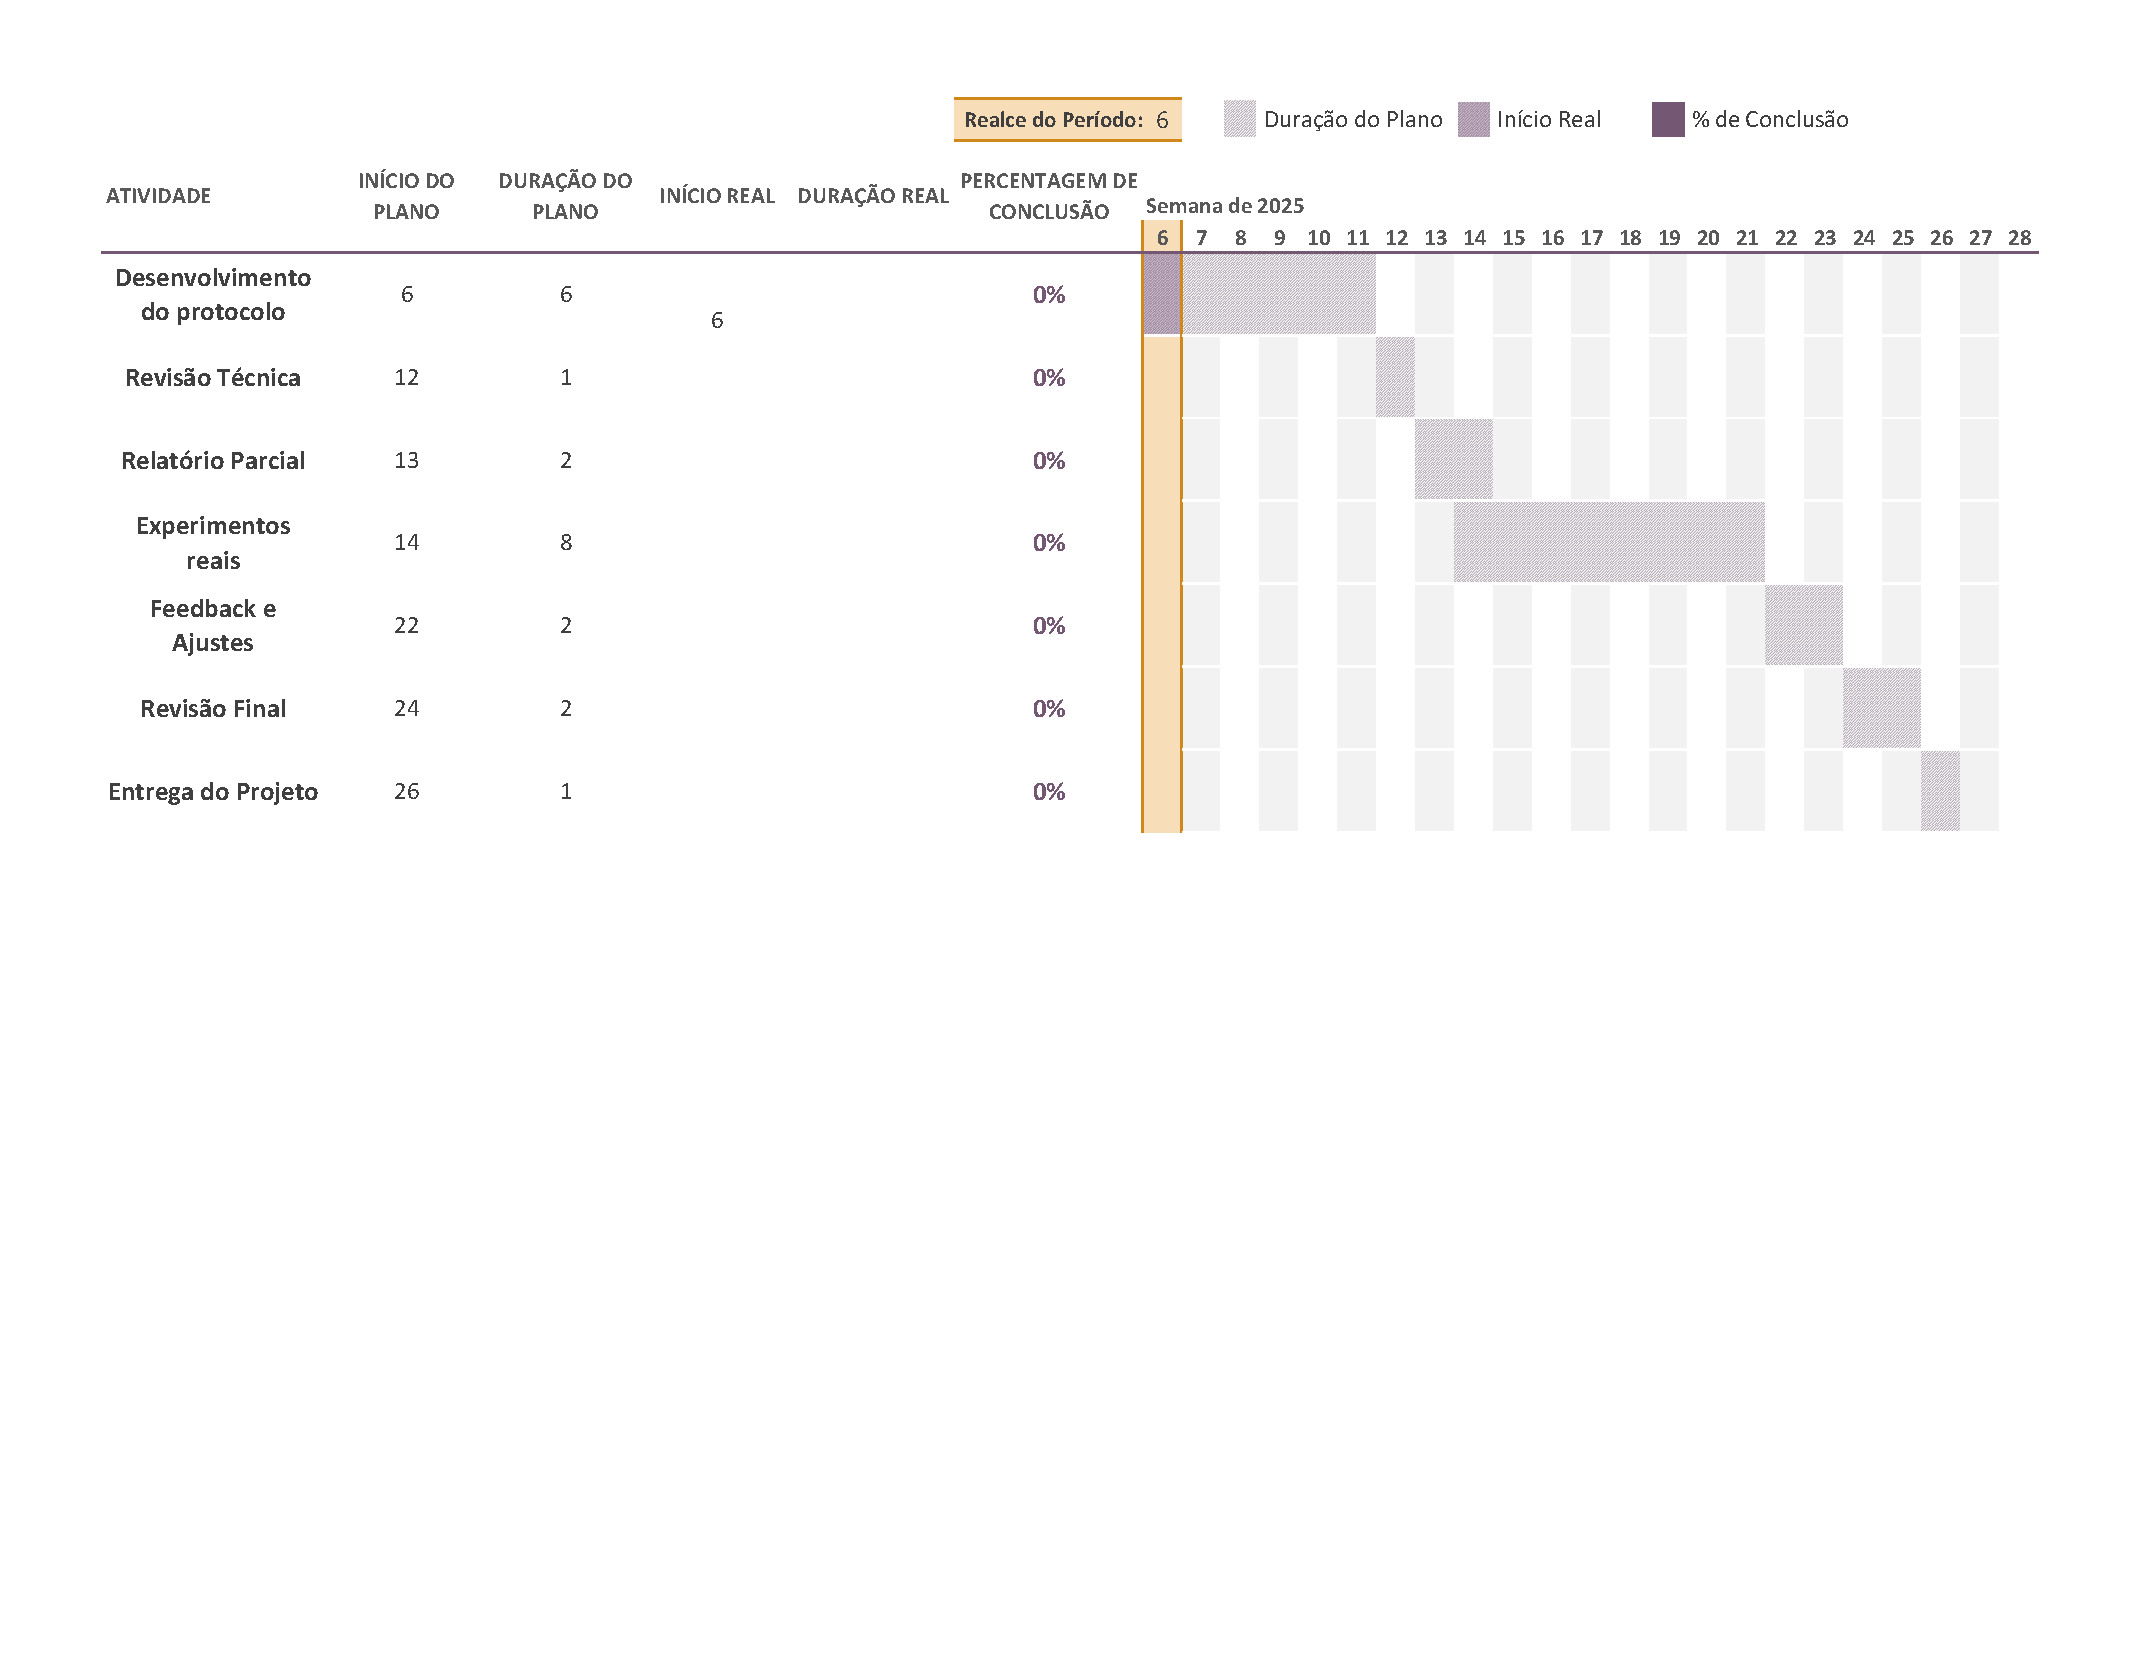
\includegraphics[width=1\linewidth]{Gantt}
  \caption{Gannt Chart.}
  \label{fig:Gannt}
\end{figure}